\documentclass[10pt]{article}
\usepackage[a4paper,margin=1cm,landscape]{geometry}
\usepackage[utf8]{inputenc}
\usepackage[french]{babel}
\usepackage{libertine}
\usepackage[T1]{fontenc}
\usepackage{xcolor}
\usepackage{tikz}
\usepackage{graphicx}

\newcommand*\circled[1]{
  \tikz[baseline=(char.base)]{
    \node[shape=circle,draw,fill=white,inner sep=2pt ] (char) {#1};}}

\title{Modèle <<Squad\footnote{Le  terme <<squad>> (traduit  ici par <<équipe>>) est le  mot utilisé  par Spotify pour  une équipe  de  développement petite, cross-fonctionnelle et  auto-organisée.}
  Health Check>> - Version française {\small basé  sur la  version 1 de  septembre 2014}}
\date{}

\begin{document}

\maketitle

\begin{tikzpicture}[remember picture, overlay]
  \node [shift={(-100 mm,-70 mm)}]  at (current page.north east) {
    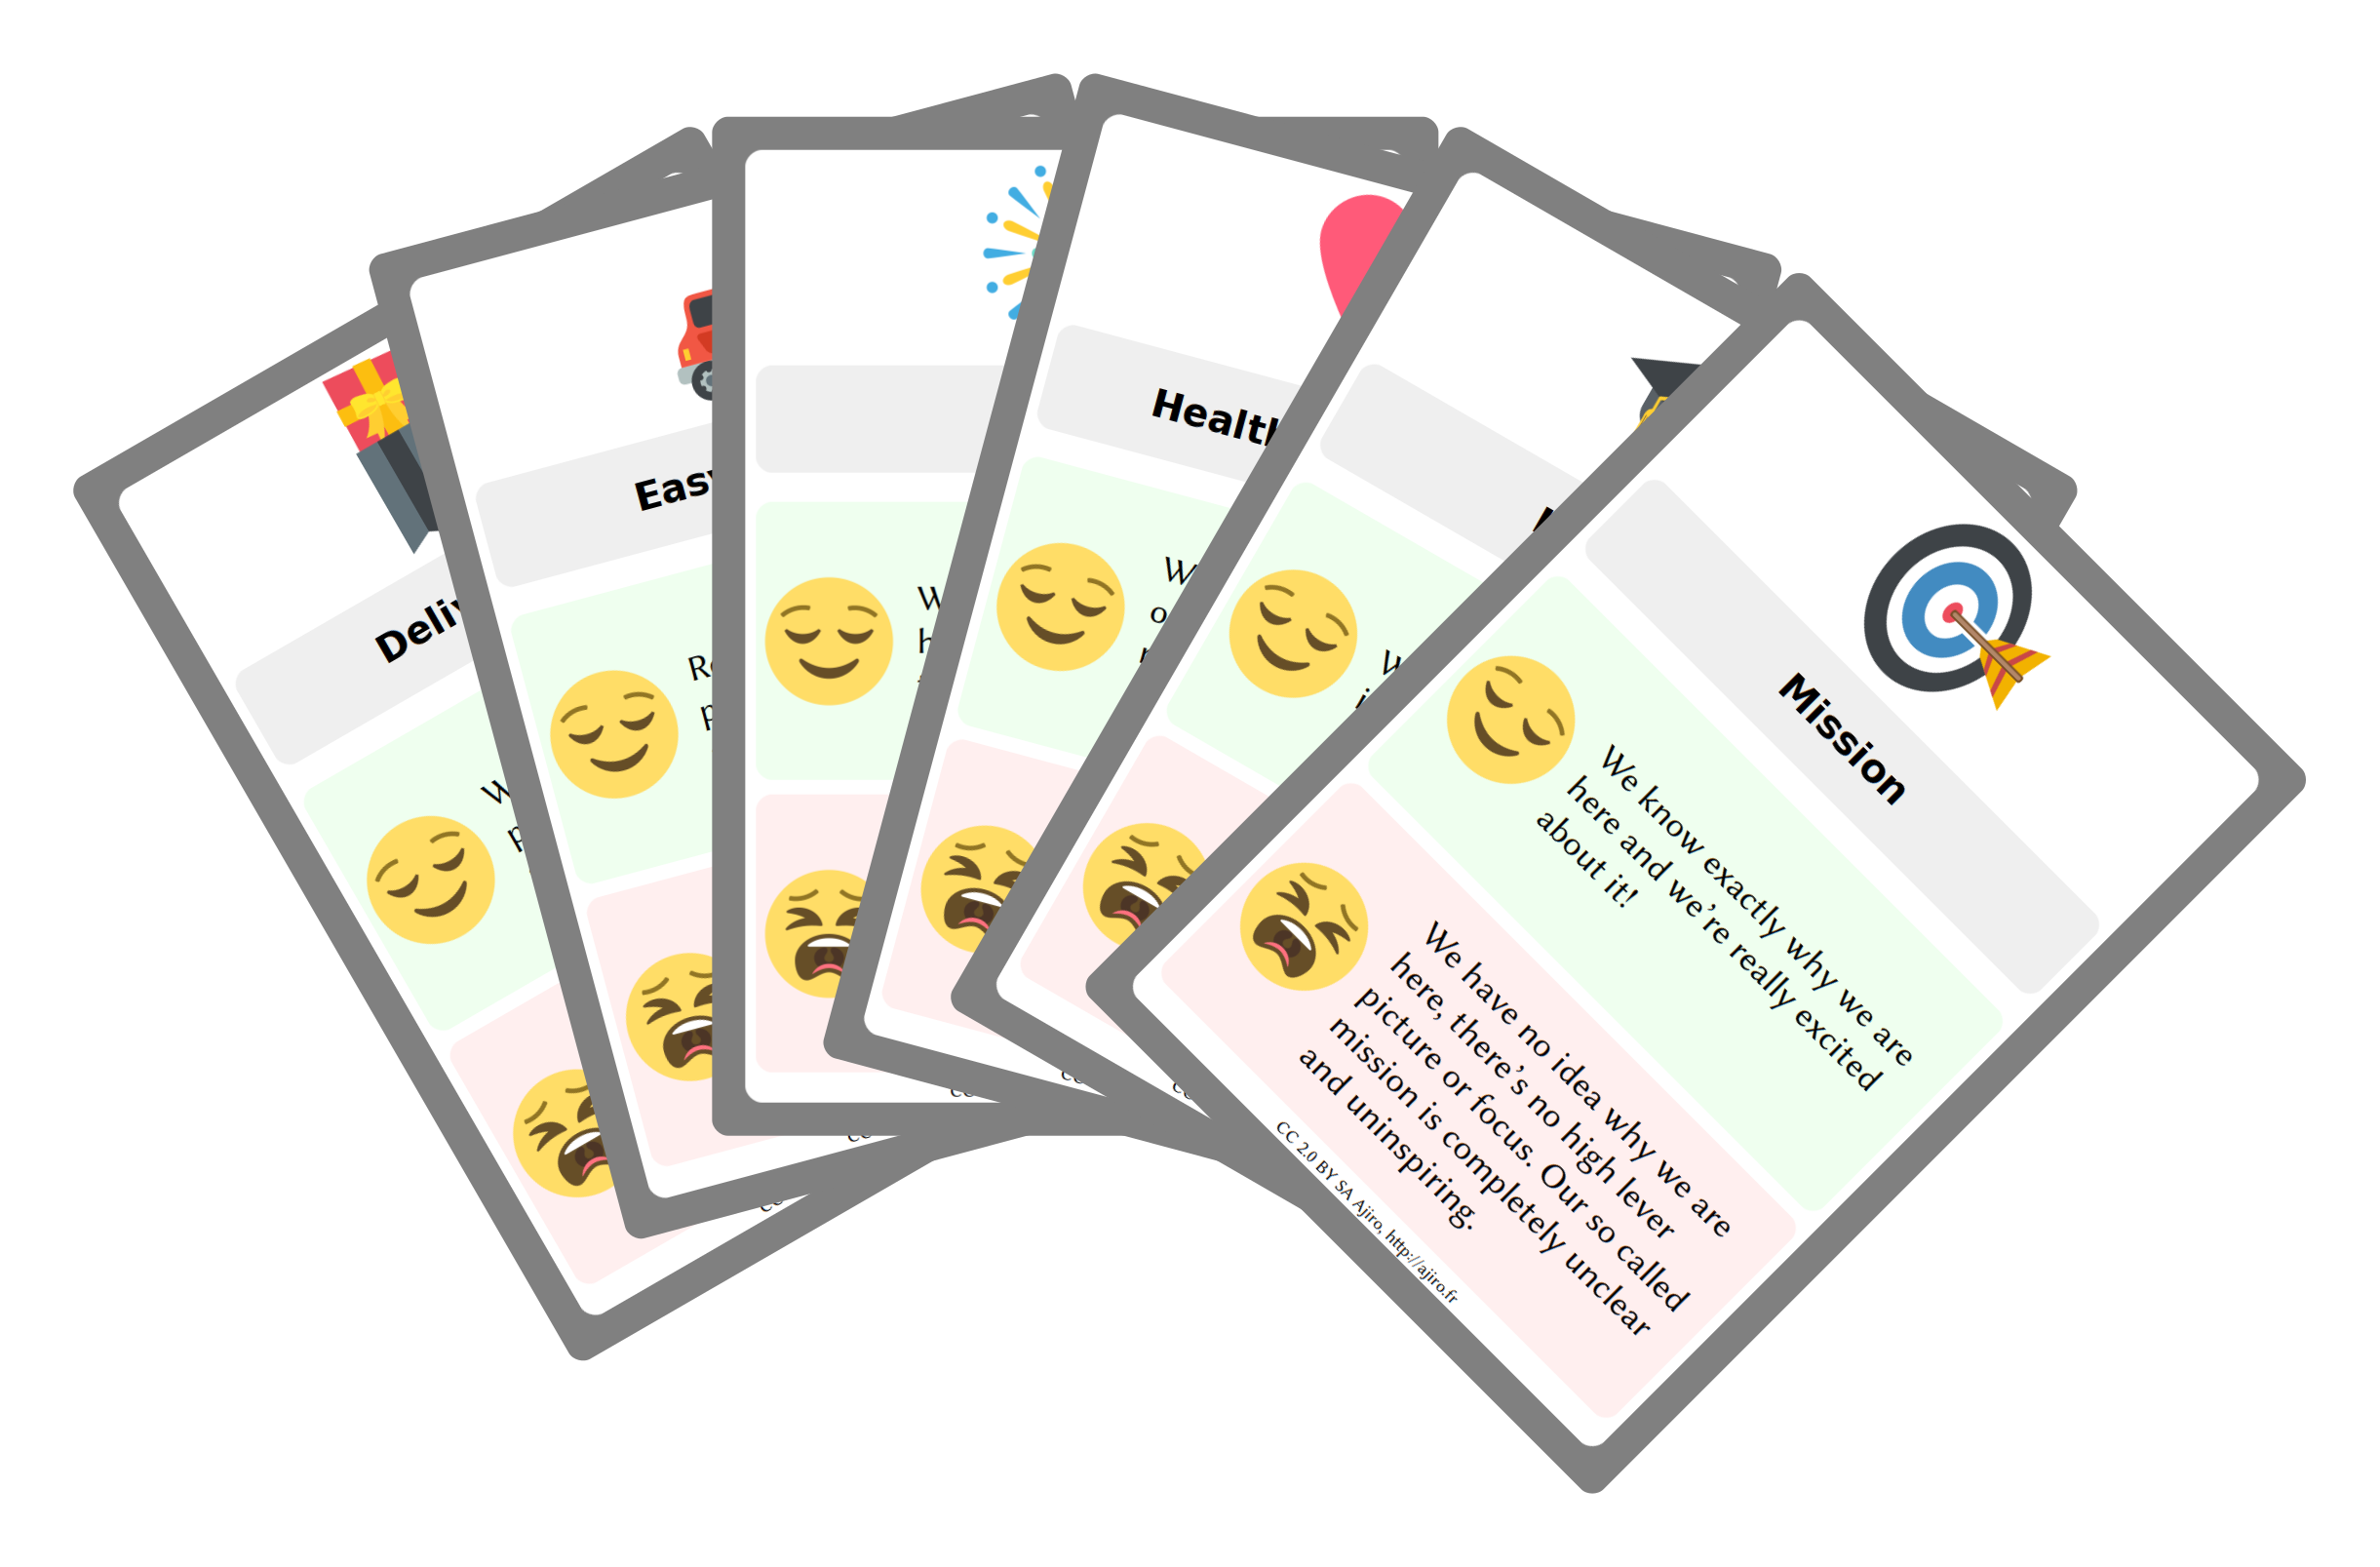
\includegraphics[width=6cm]{includes/hand}
  };
  \node [shift={(-120 mm,-85 mm)}]  at (current page.north east) {
    \Huge\circled{1}
  };
\end{tikzpicture}

\begin{tikzpicture}[remember picture, overlay]
  \node [shift={(-40 mm,-80 mm)}]  at (current page.north east) {
    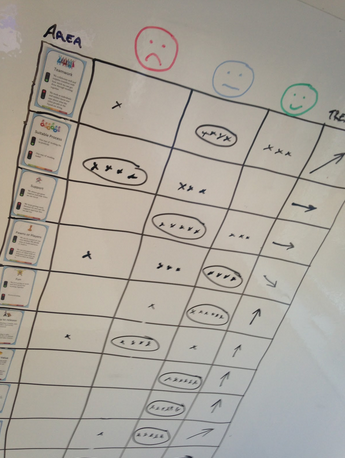
\includegraphics[width=5cm]{includes/equipe}
  };
  \node [shift={(-58 mm,-105 mm)}]  at (current page.north east) {
    \Huge\circled{2}
  };
\end{tikzpicture}

\begin{tikzpicture}[remember picture, overlay]
  \node [shift={(-54 mm,-145 mm)}]  at (current page.north east) {
    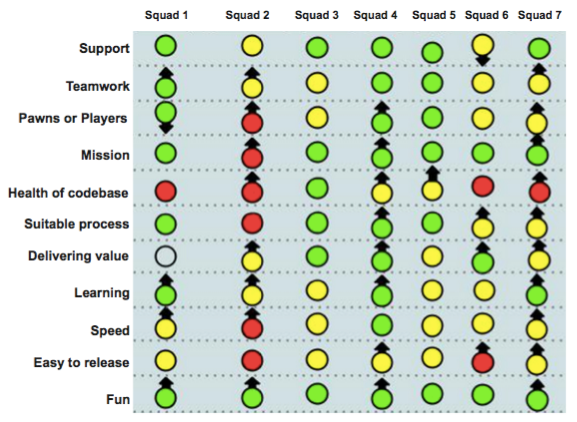
\includegraphics[width=8cm]{includes/evolution}
  };
  \node [shift={(-68 mm,-165 mm)}]  at (current page.north east) {
    \Huge\circled{3}
  };
\end{tikzpicture}

\begin{minipage}{0.6\linewidth}
\section*{De  quoi  s’agit-il ?}
Un  atelier et  une technique de  visualisation  aidant  les équipes à s’améliorer.

\section*{Audience  ?}
\begin{itemize}
  \item L’équipe  elle-même 
  \item Les personnes apportant leur  support à l’équipe
  \item (managers,  coachs, etc.) 
\end{itemize}


\section*{Comment utiliser  ce  modèle}
\begin{itemize}
  \item Rassemblez  tous  les membres de  l’équipe  dans  la  même  salle 
  \item \circled{1} : Discutez  sur les cartes  de  questions. Chacune d’entre elle  est un  indicateur  de  bonne santé,  accompagné  d’un  exemple de  très  bonne performance et  d’un  exemple particulièrement  inefficace. 
  \item \circled{2} : Demander  à l’équipe  comment elle  se  positionne sur chacun  de  ces indicateurs,  en  utilisant une méthode favorisant  les décisions de  groupe  (par  exemple : avec  les cartes  de  vote).  
  \item \circled{3} : Discutez  les tendances d’évolution de  ces indicateurs (la situation s’améliore-t-elle ? Est- elle  stable  ou  se  dégrade-t-elle  ?)
  \item Matérialisez  visuellement  les résultats de  ces discussions.  
  \item Utilisez des données quantitatives (estimation,  mesures,  extrapolation...)  pour  aider l’équipe  à s’améliorer.  
\end{itemize}


\section*{Idées de  mises en  œuvre}
  Les cartes  sont  uniquement  un  point de  départ  pour  initialiser des conversations productives. L’équipe  doit  se  sentir libre d’ajouter/ôter/modifier toute question afin  de  correspondre  à ce  qu’elle considère comme important pour  elle.

  Assurez-vous  que cet outil  soit  utilisé  en  support de  l’équipe  dans  son amélioration  et  surtout pas pour  l’évaluer!
\end{minipage} \hfill

\begin{tikzpicture}[remember picture, overlay]
  \node [shift={(-56 mm,-19 cm)}]  at (current page.north east) {
    \noindent\fcolorbox{lightgray}{lightgray}{
      \begin{minipage}{9 cm}
        \section*{\normalsize Crédits}
        \scriptsize
        \begin{itemize}
          \item Modèle  Health  check : Henrik  Kniberg \& Kristian  Lindwall,
          \item avec  l’aide  des autres  coaches agiles  chez  Spotify
          \item Design  graphique des cartes : Martin  Österberg
          \item Traduction française : Thomas  Clavier,  Séverin Legras, Hervé Taboucou, avec  l’aide  des membres d'Ajiro.fr
        \end{itemize}
        Distribuez, modifiez, réutilisez  ces contenus  sous  licence CC~BY-SA~3.0~FR
      \end{minipage}
    }
  };
\end{tikzpicture}
  

\end{document}
